%%%%%%%%%%%%%%%%%%%%%%%%%%%%%%%%%%%%%%%%%%%%%%%%%%%%%%%%%%%%%%%%%%%%%%%%%
%
% File: Model.tex
%
% Purpose: Top level document for Model.  Should not need to be edited.
%
%%%%%%%%%%%%%%%%%%%%%%%%%%%%%%%%%%%%%%%%%%%%%%%%%%%%%%%%%%%%%%%%%%%%%%%%%

\newcommand\documentHistory{
{\bf Author} & {\bf Date} & {\bf Description} \\ \hline \hline
\ModelAuthor & \ModelAuthDate & Initial Version \\ \hline
}


\documentclass[twoside,11pt,titlepage]{report}

%
% Bring in the common page setup
%
\usepackage{dynenv}

%
% Bring in the model-specific commands
%
\usepackage{gravity_torque}

%
% Bring in the graphics environment
%
\usepackage{graphicx}
\usepackage{amsmath}

%
% Bring in the hyper ref environment
%
\usepackage[colorlinks,plainpages=false]{hyperref}
%  keywords for pdfkeywords are separated by commas
\hypersetup{
   pdftitle={\gravitytorqueDesc},
   pdfauthor={\ModelAuthor},
   pdfkeywords={\ModelKeywords},
   pdfsubject={\gravitytorqueDesc}}

\begin{document}

%%%%%%%%%%%%%%%%%%%%%%%%%%%%%%%%%%%
% Front matter
%%%%%%%%%%%%%%%%%%%%%%%%%%%%%%%%%%%
\pagenumbering{roman}

\docid{models/interactions/gravity\_torque}
\docrev{1.1}
\date{\RELEASEMONTH\ \RELEASEYEAR}
\modelname{\gravitytorqueDesc}
\doctype{}
\author{\ModelAuthor}
\managers{
  Robert O. Shelton \\ Project Manager \\
  Michael T. Red \\ Simulation and Graphics Branch Chief \\
  R. Matt Ondler \\ Software, Robotics, and Simulation Division Chief}
\pdfbookmark{Title Page}{titlepage}
\makeDynenvTitlepage

\pdfbookmark{Abstract}{abstract}
%%%%%%%%%%%%%%%%%%%%%%%%%%%%%%%%%%%%%%%%%%%%%%%%%%%%%%%%%%%%%%%%%%%%%%%%
%
% Purpose: abstract for gravity torque model
%
%  
%
%%%%%%%%%%%%%%%%%%%%%%%%%%%%%%%%%%%%%%%%%%%%%%%%%%%%%%%%%%%%%%%%%%%%%%%%%

\begin{abstract}
The JEOD \gravitytorqueDesc\ computes the gravitational torque acting
on a spacecraft due to any number of gravitational bodies, both spherical
and non-spherical. The torque is computed from the gravity gradient, which
is computed by the JEOD Gravity Model.  The spacecraft mass properties,
in the form of an inertia tensor (matrix), are assumed to be known.
The total gravitational torque acting on the spacecraft is computed
in the spacecraft body-fixed frame and then transformed into the body structural frame
for output.

This document describes the implementation of the \gravitytorqueDesc.  It is part
of a series of inter-related documents that describe the model requirements,
specifications, mathematical theory, and architecture of the model.  A user
guide is also provided to assist with implementing the model in Trick
simulations.
\end{abstract}


\pdfbookmark{Contents}{contents}
\tableofcontents
\vfill

\pagebreak

%%%%%%%%%%%%%%%%%%%%%%%%%%%%%%%%%%%
% Main Document Body
%%%%%%%%%%%%%%%%%%%%%%%%%%%%%%%%%%%
\pagenumbering{arabic}

%%% For a simple document make a copy of Chapters.tex and use this format
%%% use of gravitytorqueChapters vs ModelChapters is solely for the purpose of
%%% combatability with the copy_templates.csh script.
\setcounter{chapter}{0}

%----------------------------------
\chapter{Introduction}\hyperdef{part}{intro}{}\label{ch:intro}
%----------------------------------


\section{Model Description}
%%% Incorporate the intro paragraph that used to begin this Chapter here.
%%% This is location of the true introduction where you explain why this 
%%% model exists.
%%% Identify the Model context within JEOD.

This documentation describes the design and testing of the gravity
torque routines in the JSC Engineering Orbital 
Dynamics (JEOD) \gravitytorqueDesc.  These routines 
are derived from published models that are commonly accepted in the 
aerospace industry.

Included in this documentation are verification and validation 
cases that describe tests done on the algorithms to verify that 
they are working correctly and computing the correct values for given 
input data. There is also a User Guide which describes how to incorporate the above 
mentioned routines as part of a Trick simulation.

The parent document to this model document is the
JEOD Top Level Document~\cite{dynenv:JEOD}.

\section{Document History}
%%% Status of this and only this document.  Any date should be relevant to when 
%%% this document was last updated and mention the reason (release, bug fix, etc.)
%%% Mention previous history aka JEOD 1.4-5 heritage in this section.
%%% Mention that JEOD.pdf is the parent document.

\begin{tabular}{||l|l|l|l|} \hline
\DocumentChangeHistory
\end{tabular}

\section{Document Organization}
This document is formatted in accordance with the 
NASA Software Engineering Requirements Standard~\cite{NASA:SWE} 
and is organized into the following chapters:

\begin{description}
%% longer chapter descriptions, more information.

\item[Chapter 1: Introduction] - 
This introduction contains three sections: description of model, document history, and organization.  
The first section provides the introduction to the \gravitytorqueDesc\ and its reason 
for existence.  It contains a brief description of the interconnections with other models, and 
references to any supporting documents. It also lists the document that is parent to this one.  
The second section displays the history of this document which includes
author, date, and reason for each revision.  The final
section contains a description of the how the document is organized.

\item[Chapter 2: Product Requirements] - 
Describes requirements for the \gravitytorqueDesc.

\item[Chapter 3: Product Specification] - 
Describes the underlying theory, architecture, and design of the \gravitytorqueDesc\ in detail.  It is organized in 
three sections: Conceptual Design, Mathematical Formulations, and Detailed Design.

\item[Chapter 4: User Guide] - 
Describes how to use the \gravitytorqueDesc\ in a Trick simulation.  It is broken into three sections to represent the JEOD 
defined user types: Analysts or users of simulations (Analysis), Integrators or developers of simulations (Integration),
and Model Extenders (Extension).

\item[Chapter 5: Verification and Validation] -  
Contains \gravitytorqueDesc\ verification and validation procedures and results.

\end{description}

%%%%%%%%%%%%%%%%%%%%%%%%%%%%%%%%%%%%%%%%%%%%%%%%%%%%%%%%%%%%%%%%%%%%%%%%%%%%%%%%
%%%%%%%%%%%%%%%%%%%%%%%%%%%%%%%%%%%%%%%%%%%%%%%%%%%%%%%%%%%%%%%%%%%%%%%%%%%%%%%%
%%%%%%%%%%%%%%%%%%%%%%%%%%%%%%%%%%%%%%%%%%%%%%%%%%%%%%%%%%%%%%%%%%%%%%%%%%%%%%%%
%----------------------------------
\chapter{Product Requirements}\hyperdef{part}{reqt}{}\label{ch:reqt}
%----------------------------------
The \gravitytorqueDesc\ shall meet the JEOD project requirements specified in the 
\hyperref{file:\JEODHOME/docs/JEOD.pdf}{part1}{reqt}{JEOD} top-level document.

\requirement{Gravity Gradient Matrix}
\label{reqt:gradient_matrix}
\begin{description}
\item[Requirement:]\ \newline
The gravity gradient shall be modeled as a 3x3 Jacobian (matrix) that is
the partial derivative of the gravity acceleration vector with respect to
position in rectangular inertial coordinates. 
\item[Rationale:]\ \newline



The JEOD
\hyperref{file:\JEODHOME/models/environment/gravity/docs/gravity.pdf}{}{}
{Gravity Model} computes the gravity gradient for all 
gravitational bodies as a 3x3 Jacobian (matrix).  
\item[Verification:]\ \newline
Inspection
\end{description}

\requirement{Spacecraft Mass Properties}
\label{reqt:mass_properties}
\begin{description}
\item[Requirement:]\ \newline
The mass properties of any spacecraft shall be modeled as a 3x3 inertia
tensor (matrix) expressed in the spacecraft body-fixed coordinate system.
\item[Rationale:]\ \newline
A 3x3 inertia tensor is the widely accepted industry standard for 
representing the mass properties of any rigid body, and JEOD uses
this representation.
\item[Verification:]\ \newline
Inspection
\end{description}

\requirement{Spacecraft Attitude}
\label{reqt:spacecraft_attitude}
\begin{description}
\item[Requirement:]\ \newline
The attitude representation of any spacecraft shall 
represent a transformation from inertial coordinates
to spacecraft body-fixed coordinates.
\item[Rationale:]\ \newline
The mass properties of the spacecraft are expressed in spacecraft 
body-fixed coordinates. The gravity gradient matrix is expressed in
inertial coordinates.  In order to compute the gravity 
torque on the spacecraft in the body-fixed system, the attitude of the spacecraft must be
known (inertial to body-fixed).
\item[Verification:]\ \newline
Inspection
\end{description}

%\label{sec:func_reqts}
%This section identifies requirements on the functional capabilities
%of the \gravitytorqueDesc.
\requirement{Gravity Torque}
\label{reqt:gravity_torque}
\begin{description}
\item[Requirement:]\ \newline
The model shall compute the inertial torque vector acting on a spacecraft from 
a gravity gradient Jacobian matrix, an inertia tensor (matrix), and
the spacecraft attitude.
   \subrequirement{}
   The torque vector shall be expressed in the spacecraft body-fixed coordinate system.
The torque vector is output in the structural reference frame.
\item[Rationale:]\ \newline
The gravity torque acting on a spacecraft affects the attitude of the spacecraft
and must be modeled for accurate simulations.
\item[Verification:]\ \newline
Test
\end{description}

%%% Format for the model Requirements is open.  It should include requirements for this model 
%%% only and use requirment tags like the one below.
%\requirement{...}
%\label{reqt:...}
%\begin{description}
%  \item[...]\ \newline
%    The documentation for the model shall include
%
%    \subrequirement{}
%    \label{reqt:...}
%      Software requirements specification.
%      
%    ...
%   
%  \item[title]\ \newline
%    text
%
%  ...
%
%\end{description}


%%%%%%%%%%%%%%%%%%%%%%%%%%%%%%%%%%%%%%%%%%%%%%%%%%%%%%%%%%%%%%%%%%%%%%%%%%%%%%%%
%%%%%%%%%%%%%%%%%%%%%%%%%%%%%%%%%%%%%%%%%%%%%%%%%%%%%%%%%%%%%%%%%%%%%%%%%%%%%%%%
%%%%%%%%%%%%%%%%%%%%%%%%%%%%%%%%%%%%%%%%%%%%%%%%%%%%%%%%%%%%%%%%%%%%%%%%%%%%%%%%
%----------------------------------
\chapter{Product Specification}\hyperdef{part}{spec}{}\label{ch:spec}
%----------------------------------

\section{Conceptual Design}
The \gravitytorqueDesc\ is a function that computes torque
due to gravity gradient acting on a spacecraft. The model is not a stand-alone 
function. It requires the spacecraft mass properties (inertia tensor) and the 
gravity gradient (at the spacecraft's current location) to be computed
before calling the \gravitytorqueDesc. The gravity gradient is computed
by the JEOD Gravity Model and is used
to compute the force of gravity acting on each infinitesimal mass of the
spacecraft body, as defined by the spacecraft inertia tensor. 
The forces, in combination with the mass distribution,
are combined to form the total gravity torque acting on the spacecraft.

The \gravitytorqueDesc\ is based on the derivation and Ada code 
of Gottlieb\cite{JSC23762}. Sign changes have been made to the inertia
tensor in order to be compatible with other JEOD models and to be consistent with 
aerospace industry standards.\footnote{Gottlieb's Ada code (\cite{JSC23762} p.49) contains
sign changes compared to his equations on p.21-23. The signs in the
\gravitytorqueDesc\ formulation match Gottlieb's Ada code.}

%%***INSERT DIAGRAM SHOWING INTERACTION WITH OTHER JEOD MODELS***

%%%%%%%%%%%%%%%%%%%%%%%%%%%%%%%%%%%%%%%%%%%%%%%%%%%%%%%%%%%%%%%%%%%%%%%%%%%%%%%%
\section{Mathematical Formulations}

\subsection{Gravity Gradient}
The gravity gradient is a 3x3 Jacobian (matrix) that is the partial derivative
of the inertial gravitational acceleration vector with respect to the inertial
position vector (rectangular coordinates).
\begin{equation}
\nabla \bar{a} = \frac{\partial\bar{a}}{\partial\bar{r}} = 
\left[
\begin{array}{ccc}
\partial{a_x}/\partial{x} & \partial{a_x}/\partial{y} & \partial{a_x}/\partial{z} \\
\partial{a_y}/\partial{x} & \partial{a_y}/\partial{y} & \partial{a_y}/\partial{z} \\
\partial{a_z}/\partial{x} & \partial{a_z}/\partial{y} & \partial{a_z}/\partial{z} \\
\end{array}
\right]
\end{equation}

The trace of the gravity gradient (sum of the diagonal terms) is the Laplacian of
the gravitational potential and will be 
equal to zero for any gravity field.
\begin{equation}
\nabla^2 V = \frac{\partial^2V}{\partial x^2}+\frac{\partial^2V}{\partial y^2}+\frac{\partial^2V}{\partial z^2} =
\frac{\partial a_x}{\partial x}+\frac{\partial a_y}{\partial y}+\frac{\partial a_z}{\partial z} = 0
\end{equation}
where $V$ is the gravitational potential\cite{kaula1966}.


\subsection{Spacecraft Mass Properties - Inertia Tensor}
The mass properties (i.e., mass distribution) of a rigid body can be expressed as 
a tensor (matrix) in the spacecraft body-fixed coordinate system as
\begin{equation}
I = 
\left[
\begin{array}{rrr}
 I_{xx} &  I_{xy} &  I_{xz} \\
 I_{xy} &  I_{yy} &  I_{yz} \\
 I_{xz} &  I_{yz} &  I_{zz} \\
\end{array}
\right]
\end{equation}
where

\begin{equation}
\begin{aligned}
I_{xx}  &= \int_B (\rho_y^2+\rho_z^2) dm\\
I_{yy}  &= \int_B (\rho_x^2+\rho_z^2) dm\\
I_{zz}  &= \int_B (\rho_x^2+\rho_y^2) dm\\
\end{aligned}
\end{equation}
are the moments of intertia, and
\begin{equation}
\begin{aligned}
I_{xy}  &= \int_B (-\rho_x\rho_y) dm\\
I_{xz}  &= \int_B (-\rho_x\rho_z) dm\\
I_{yz}  &= \int_B (-\rho_y\rho_z) dm\\
\end{aligned}
\end{equation}
are the products of inertia\cite{kaplan1976}. The vector $\bar{\rho}$, whose
components are $\rho_x$, $\rho_y$, $\rho_z$, locates each infinitesimal mass
of the spacecraft 
in the body-fixed system. The integrals are computed
over the entire spacecraft body in the spacecraft 
body-fixed frame. Therefore, the inertia tensor is
also expressed in the body-fixed frame.


\subsection{Gravity Torque}
The gravity gradient matrix can be transformed from inertial 
coordinates to spacecraft body-fixed coordinates using a similarity transformation\cite{SJ}.
\begin{equation}\label{eqn:G}
G = B\frac{\partial\bar{a}}{\partial\bar{r}} B^T
\end{equation}
where $B$ is the inertial to body-fixed attitde matrix.

The gravitational torque acting on the spacecraft can then be expressed as\cite{JSC23762}
\begin{equation}
\bar{\tau} = \int \bar{\rho}\times G \bar{\rho} dm
\end{equation}
The vector $\bar{\rho}$ is defined in the previous section.
The torque can be expressed in terms of $I$ and $G$ as
\begin{equation}
\bar{\tau} = \left[
\begin{array}{c}
G_{2,3}(I_{zz}-I_{yy}) - G_{1,3}I_{xy} + G_{1,2}I_{xz} - I_{yz}(G_{3,3}-G_{2,2}) \\
G_{1,3}(I_{xx}-I_{zz}) + G_{2,3}I_{xy} - G_{1,2}I_{yz} - I_{xz}(G_{1,1}-G_{3,3}) \\
G_{1,2}(I_{yy}-I_{xx}) - G_{2,3}I_{xz} + G_{1,3}I_{yz} - I_{xy}(G_{2,2}-G_{1,1}) \\
\end{array}
\right]
\end{equation}
See Gottlieb\cite{JSC23762} (p.21-23) for details.
The final gravity gradient torques are output in the structural reference frame.

%%%%%%%%%%%%%%%%%%%%%%%%%%%%%%%%%%%%%%%%%%%%%%%%%%%%%%%%%%%%%%%%%%%%%%%%%%%%%%%%
\section{Detailed Design}
The \gravitytorqueDesc\ was adopted from Gottlieb's Ada
code (see Gottlieb\cite{JSC23762} p.49).  The inertia tensor $I$ and the 
gravity gradient $G$ are computed in JEOD by the Dynamics Manager
and the Gravity Model.
Gottlieb's derivation and Ada code assume the attitude matrix $B$ transforms
from body-fixed to earth-fixed coordinates.  In JEOD, the $B$ matrix transforms
from inertial to body-fixed coordinates, so a change from Gottlieb's derivation
in equation \ref{eqn:G} was needed.  Details of the derivation
of the model are shown in \cite{JSC23762} and are not repeated here.
Details of the design in the \gravitytorqueDesc\ can be found in
\href{file:refman.pdf}
{JEOD Gravity Torque Model Reference Manual}~\cite{gravtorq_refman}.

%%%%%%%%%%%%%%%%%%%%%%%%%%%%%%%%%%%%%%%%%%%%%%%%%%%%%%%%%%%%%%%%%%%%%%%%%%%%%%%%
%%%%%%%%%%%%%%%%%%%%%%%%%%%%%%%%%%%%%%%%%%%%%%%%%%%%%%%%%%%%%%%%%%%%%%%%%%%%%%%%
%%%%%%%%%%%%%%%%%%%%%%%%%%%%%%%%%%%%%%%%%%%%%%%%%%%%%%%%%%%%%%%%%%%%%%%%%%%%%%%%
%----------------------------------
\chapter{User Guide}\hyperdef{part}{user}{}\label{ch:user}
%----------------------------------
The Analysis section of the user guide is intended primarily for users of pre-existing simulations.  
It contains: 
\begin{itemize}
\item A description of how to modify \gravitytorqueDesc\ variables after the simulation 
has compiled, including an in-depth discussion of the input file,
\item An overview of how to interpret (but not edit) the S\_define file,
\item A sample of some of the typical variables that may be logged.
\end{itemize}

The Integration section of the user guide is intended for simulation developers.  
It describes the necessary configuration of the \gravitytorqueDesc\ within an 
S\_define file, and the creation of standard run directories.  The latter 
component assumes a thorough understanding of the preceding Analysis section of the user guide.
Where applicable, the user may be directed to selected portions of Product Specification (Chapter \ref{ch:spec}).

The Extension section of the user guide is intended primarily for developers 
needing to extend the capability of the \gravitytorqueDesc.  Such users should have a 
thorough understanding of how the model is used in the preceding 
Integration section, and of the model 
specification (described in Chapter \ref{ch:spec}).

%%%%%%%%%%%%%%%%%%%%%%%%%%%%%%%%%%%%%%%%%%%%%%%%%%%%%%%%%%%%%%%%%%%%%%%%%%%%%%%%
\section{Analysis}

\subsection{Using the \gravitytorqueDesc\ }
The mass properties of a spacecraft must
first be defined in the form of an inertia tensor (matrix).  An example of 
configuring the inertia tensor of a spacecraft (sim object) named VEH\_OBJ is:
\begin{verbatim}
VEH_OBJ.mass_init.properties.mass             {kg} =  400000.0;
VEH_OBJ.mass_init.properties.position[0]       {M} = -3.0, -1.5, 4.0;
VEH_OBJ.mass_init.properties.inertia[0][0] {kg*M2} =  1.02e+8,-6.96e+6,-5.48e+6;
VEH_OBJ.mass_init.properties.inertia[1][0] {kg*M2} = -6.96e+6, 0.91e+8, 5.90e+5;
VEH_OBJ.mass_init.properties.inertia[2][0] {kg*M2} = -5.48e+6, 5.90e+5, 1.64e+8;
\end{verbatim}

In order to compute gravity torque, the {\it gradient} flag must be set in the
gravity controls for each spacecraft and each gravitational body (i.e., planet) desired.
Setting the gradient flag to ``false" for a particular planet will result in the 
null matrix, thus removing that planet's contribution to the overall
gravitational torque.  An example of setting this flag to true for a spacecraft 
called VEH\_OBJ for the planet Earth is:
\begin{verbatim}
VEH_OBJ.grav_controls[GC_EARTH].gradient        = true;
VEH_OBJ.grav_controls[GC_EARTH].gradient_degree = 5;
VEH_OBJ.grav_controls[GC_EARTH].gradient_order  = 5;
\end{verbatim}

The degree and order of the gravity gradient torque can be set independently
of the acceleration degree and order for each gravitational body for each
spacecraft. The gradient degree and order must be less
than or equal to the acceleration degree and order. 
In the example above, the 
gradient degree and order are both 5.
If the gradient degree and order are not specified,
JEOD will compute the spherical body gradient as a default.
Spherical body gradient can also be invoked by setting the gradient
degree and order both to 0. 

An example of setting the Earth gravity accleration degree to 70 and the
order to 70 for a single spacecraft is:
\begin{verbatim}
VEH_OBJ.grav_controls[GC_EARTH].degree    = 70;
VEH_OBJ.grav_controls[GC_EARTH].order     = 70;
\end{verbatim}

Any gravitational body can be modeled as a perfect sphere to simplify and
speed up gravity computations. Setting the gravity field to {\it spherical} will
also cause the gravity gradient to be based on the gravity of a spherical body.
An example of setting a gravitational body to spherical is:
\begin{verbatim}
VEH_OBJ.grav_controls[GC_EARTH].spherical = true;
\end{verbatim}
If a body is set to spherical, the gravity degree and order are forced to be
zero (by definition).  As previously mentioned, spherical body gradient can
also be invoked by setting the gradient degree and order both to 0.


\subsection{How to Interpret the S\_define File}
Each spacecraft (sim object) requires its own structure for computing gravity torque.  
This structure will be of type ``GravityTorque" and declared in the S\_define file. 
The gravity torque function is initialized with a call to the function grad\_torque.initialize.
At the desired job cycle rate, the gravity torque is computed (updated) by a call to the
function grad\_torque.update. The resulting torque is accumulated by a vcollect statement in 
the S\_define file. 

\subsection{Data Logging}
For logging the gravity torque acting on any spacecraft, include a line similar to this in the log 
setup file that is used to log forces and torques:
\begin{verbatim}
   "#(VEH_OBJ).grav_torque.torque[0-2]",
\end{verbatim}
The exact name of the variable to be logged will depend on the structure
declaration for each spacecraft.  Details can be found in the next section.

%%%%%%%%%%%%%%%%%%%%%%%%%%%%%%%%%%%%%%%%%%%%%%%%%%%%%%%%%%%%%%%%%%%%%%%%%%%%%%%%
\section{Integration}

In the S\_define file, for each vehicle object, include this structure:
\begin{verbatim}
   interactions/gravity_torque: GravityTorque grav_torque;
\end{verbatim}

Include this initialization job (sv\_dyn is the vehicle sim object in this example):
\begin{verbatim}
   (initialization) interactions/gravity_torque:
      sv_dyn.grad_torque.initialize( In DynBody & subject = sv_dyn.body );
\end{verbatim}

Include this derivative class job:
\begin{verbatim}
   P_BODY Idynamics (derivative) interactions/gravity_torque:
      sv_dyn.grav_torque.update();
\end{verbatim}

Include grad\_torque in the non-transmitted torque collection for each vehicle. An example
that also includes aerodynamic torque is:
\begin{verbatim}
vcollect sv_dyn.body.collect.collect_no_xmit_torq CollectTorque::create {
   sv_dyn.aero_drag.aero_torque,
   sv_dyn.grav_torque.torque
};
\end{verbatim}

Gravity gradient must be made active in the gravity controls for each vehicle (and
each gravitational body) in the simulation input file or in a modified data 
file.  The gradient degree and order can be specified separately from the acceleration
degree and order. An example is shown below. If not specified, the default gravity
gradient will be that due to a spherical body.
\begin{verbatim}
/* Configure gravity gradient torque. */
VEH_OBJ.grav_torque.active = true;

/* Set up the gravity controls for the Earth. */
VEH_OBJ.grav_controls[0].source_name     = "Earth";
VEH_OBJ.grav_controls[0].active          = true;
VEH_OBJ.grav_controls[0].spherical       = false;
VEH_OBJ.grav_controls[0].degree          = 36;
VEH_OBJ.grav_controls[0].order           = 36;
VEH_OBJ.grav_controls[0].gradient        = true;
VEH_OBJ.grav_controls[0].gradient_degree = 5;
VEH_OBJ.grav_controls[0].gradient_order  = 5;
\end{verbatim}
The last three lines in this set activate the gravity gradient and set the degree
and order both to 5. Setting the gradient flag to ``false" will result in the null 
matrix being computed for the gravity gradient. 


%%%%%%%%%%%%%%%%%%%%%%%%%%%%%%%%%%%%%%%%%%%%%%%%%%%%%%%%%%%%%%%%%%%%%%%%%%%%%%%%
\section{Extension}
The \gravitytorqueDesc\ is a function based directly on first principles
of physics/dynamics.  Therefore, the model is not extensible.


%%%%%%%%%%%%%%%%%%%%%%%%%%%%%%%%%%%%%%%%%%%%%%%%%%%%%%%%%%%%%%%%%%%%%%%%%%%%%%%%
%%%%%%%%%%%%%%%%%%%%%%%%%%%%%%%%%%%%%%%%%%%%%%%%%%%%%%%%%%%%%%%%%%%%%%%%%%%%%%%%
%%%%%%%%%%%%%%%%%%%%%%%%%%%%%%%%%%%%%%%%%%%%%%%%%%%%%%%%%%%%%%%%%%%%%%%%%%%%%%%%
%----------------------------------
\chapter{Verification and Validation}\hyperdef{part}{ivv}{}\label{ch:ivv}
%----------------------------------

\section{Verification}\label{sec:verif}
%%% code imported from old template structure
%\inspection{<Name of Inspection>}\label{inspect:<label>}
% <description> to satisfy  
% requirement \ref{reqt:<label>}.

The \gravitytorqueDesc\ was verified for the spherical body case by comparing
the model results with the analytical results for spherical body gravity 
gradient torque. The analytical expression for spherical body torque 
expressed in the spacecraft body frame is\cite{SJ}
\begin{equation}\label{eqn:spherical_torque}
\bar{\tau}=\frac{3\mu}{r^5} \left(\bar{r}\times I \bar{r}\right)
\end{equation}
where $I$ is the inertia matrix in the spacecraft body frame, and the 
vector $\bar{r}$ has been transformed into the spacecraft body frame.

Six separate runs of the SIM\_torque\_compare\_simple simulation of a low 
Earth orbiting satellite were executed to verify the functionality
of the \gravitytorqueDesc. In the first run (RUN\_01), the
Earth was specified to be a spherical body and the gravity gradient was
\emph{not} activated using these lines in the input file:
\begin{verbatim}
/* Set up the gravity controls for the Earth. */
VEH_OBJ.grav_controls[0].source_name     = "Earth";
VEH_OBJ.grav_controls[0].active          = true;
VEH_OBJ.grav_controls[0].spherical       = true;
VEH_OBJ.grav_controls[0].degree          = 20;
VEH_OBJ.grav_controls[0].order           = 20;
VEH_OBJ.grav_controls[0].gradient        = false;
VEH_OBJ.grav_controls[0].gradient_degree = 0;
VEH_OBJ.grav_controls[0].gradient_order  = 0;
\end{verbatim}
With the gradient set to false, the \gravitytorqueDesc\ computed zero torque.
The results are shown in the figure \ref{fig:run01_results}, where 
the ``benchmark" curve is a plot of the analytical results of 
equation \ref{eqn:spherical_torque}.  As expected, the
computed torque was zero in all three body frame directions.
\begin{figure}[h!]
\centering
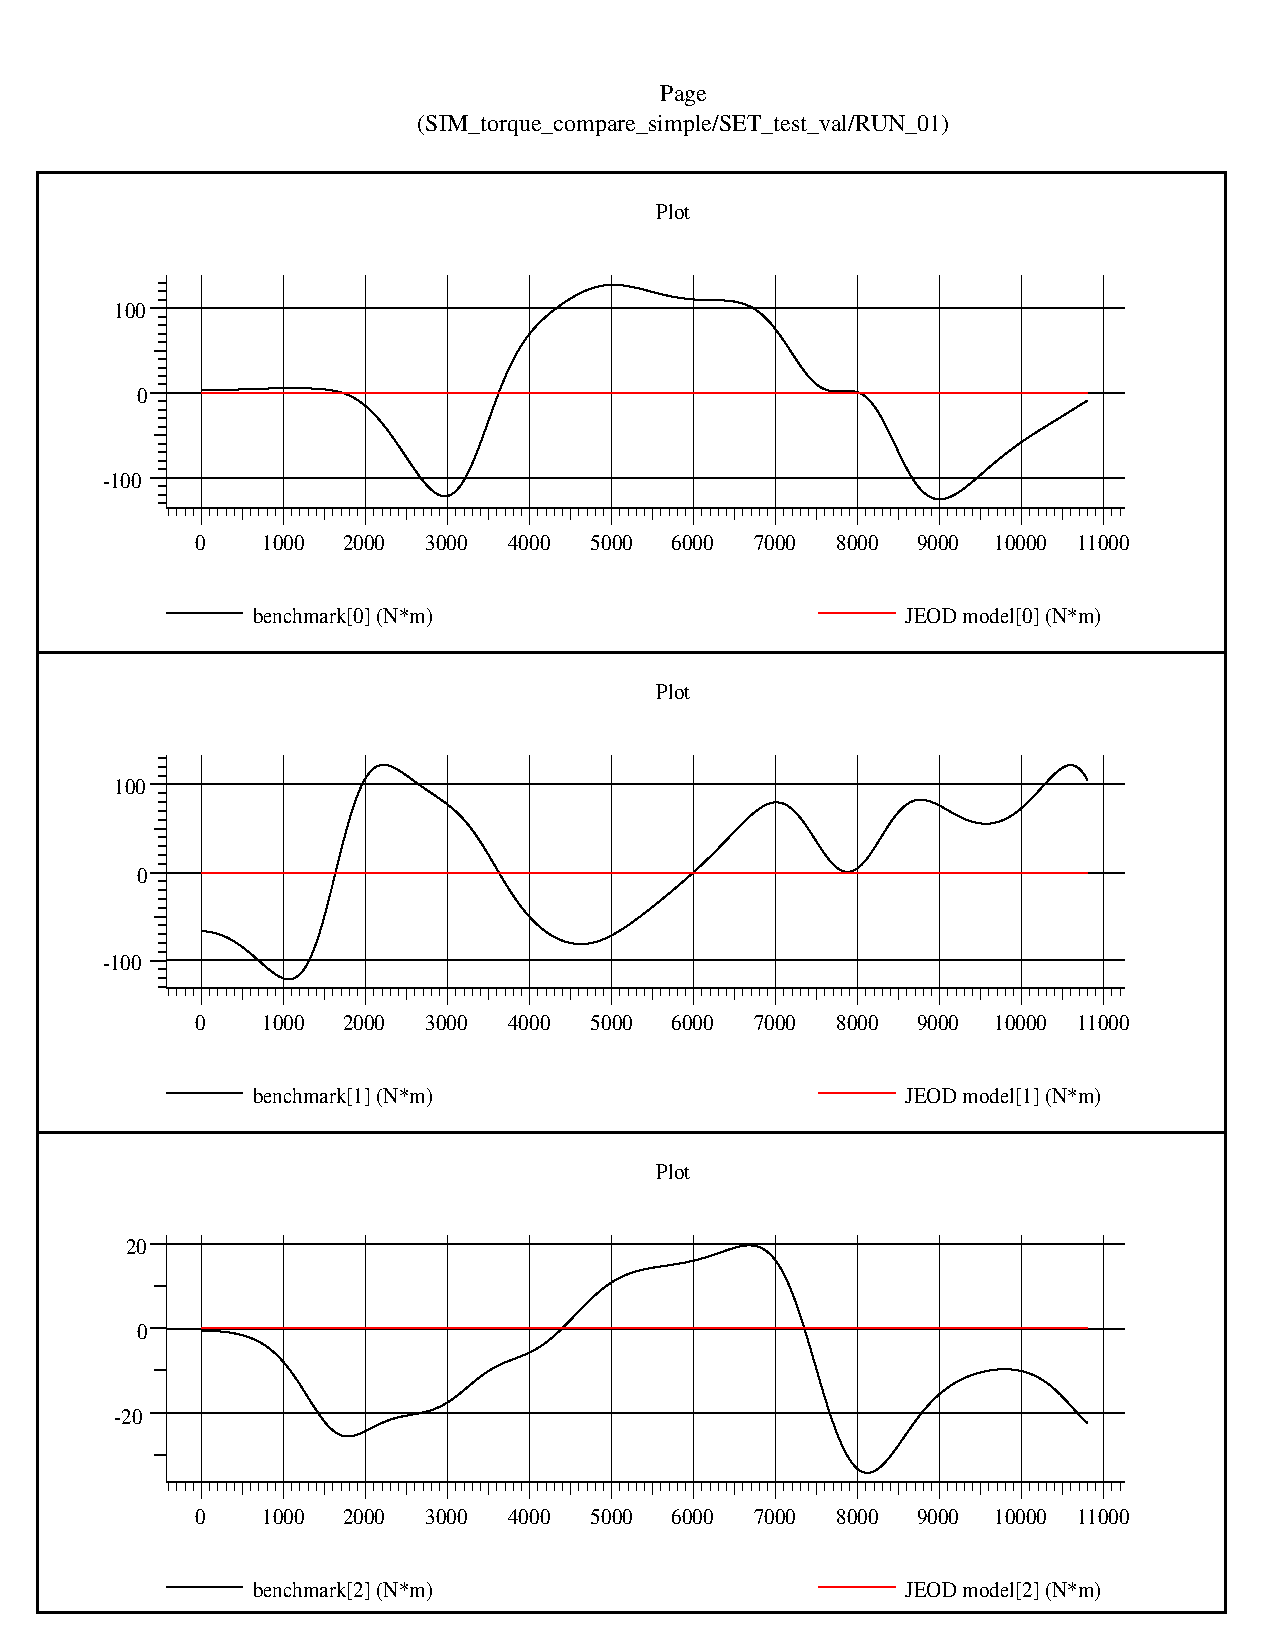
\includegraphics[width=6.1in]{figs/run_01.pdf}
\caption{RUN\_01 results.}
\label{fig:run01_results}
\end{figure}
\newpage

In the second sim run (RUN\_02), the Earth was specified to be a
spherical body and the gravity gradient was activated using these 
lines in the input file:
\begin{verbatim}
/* Set up the gravity controls for the Earth. */
VEH_OBJ.grav_controls[0].source_name     = "Earth";
VEH_OBJ.grav_controls[0].active          = true;
VEH_OBJ.grav_controls[0].spherical       = true;
VEH_OBJ.grav_controls[0].degree          = 20;
VEH_OBJ.grav_controls[0].order           = 20;
VEH_OBJ.grav_controls[0].gradient        = true;
VEH_OBJ.grav_controls[0].gradient_degree = 0;
VEH_OBJ.grav_controls[0].gradient_order  = 0;
\end{verbatim}
The results are shown in the figure \ref{fig:run02_results}.
Again, the ``benchmark" curve is a plot of the analytical results of 
equation \ref{eqn:spherical_torque}.  As expected, the
computed torque was equal to the analytical spherical body
torque in all three body frame directions.
\begin{figure}[h!]
\centering
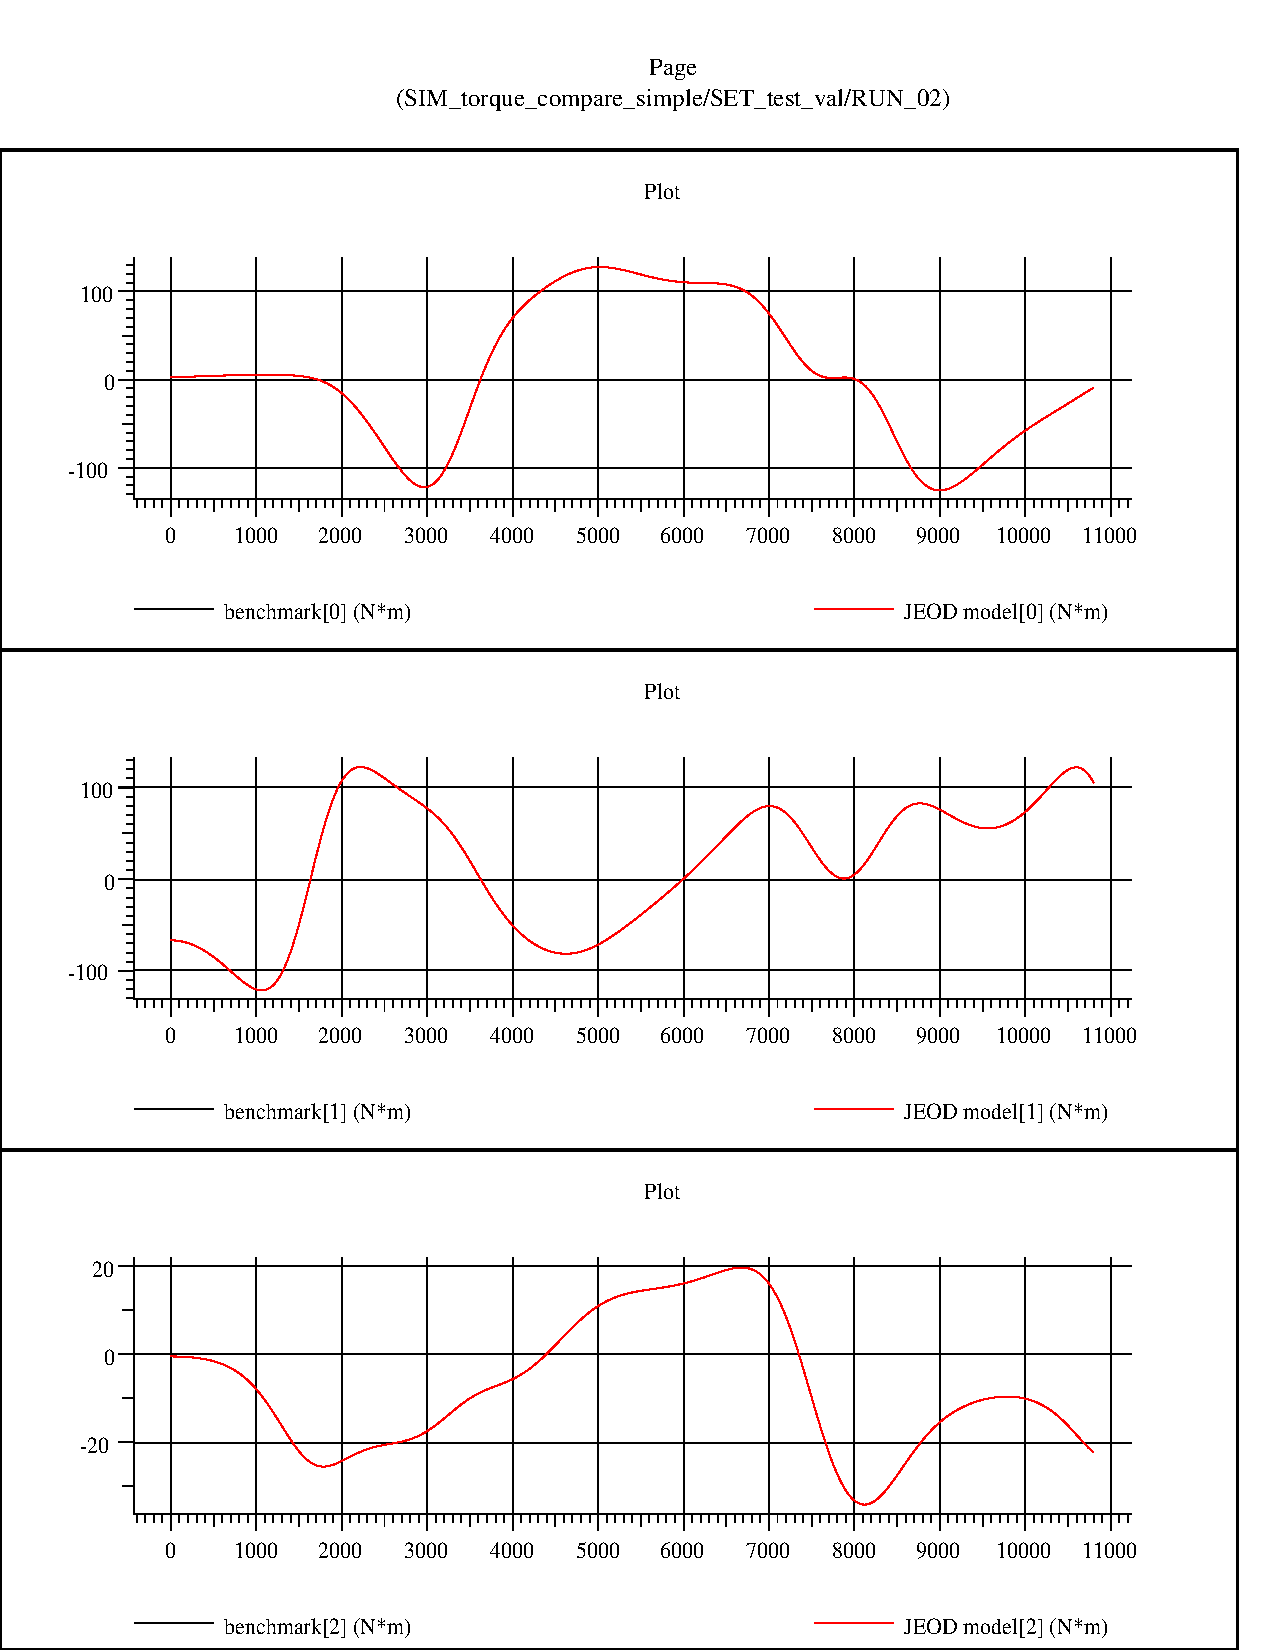
\includegraphics[width=6.1in]{figs/run_02.pdf}
\caption{RUN\_02 results.}
\label{fig:run02_results}
\end{figure}
\newpage

In the third sim run (RUN\_03), the Earth was  was specified to be a
spherical body and the gravity gradient was activated.  The gravity
gradient degree and order were both specified to be 4 using these 
lines in the input file:
\begin{verbatim}
/* Set up the gravity controls for the Earth. */
VEH_OBJ.grav_controls[0].source_name     = "Earth";
VEH_OBJ.grav_controls[0].active          = true;
VEH_OBJ.grav_controls[0].spherical       = true;
VEH_OBJ.grav_controls[0].degree          = 20;
VEH_OBJ.grav_controls[0].order           = 20;
VEH_OBJ.grav_controls[0].gradient        = true;
VEH_OBJ.grav_controls[0].gradient_degree = 4;
VEH_OBJ.grav_controls[0].gradient_order  = 4;
\end{verbatim}
The results are shown in the figure \ref{fig:run03_results}.
Even though the gradient degree and order were specified for a non-spherical
body, the spherical gradient was computed because the Earth was
specified to be a spherical body.  
The resulting torque was equal to the analytical spherical body
torque in all three body frame directions.
\begin{figure}[h!]
\centering
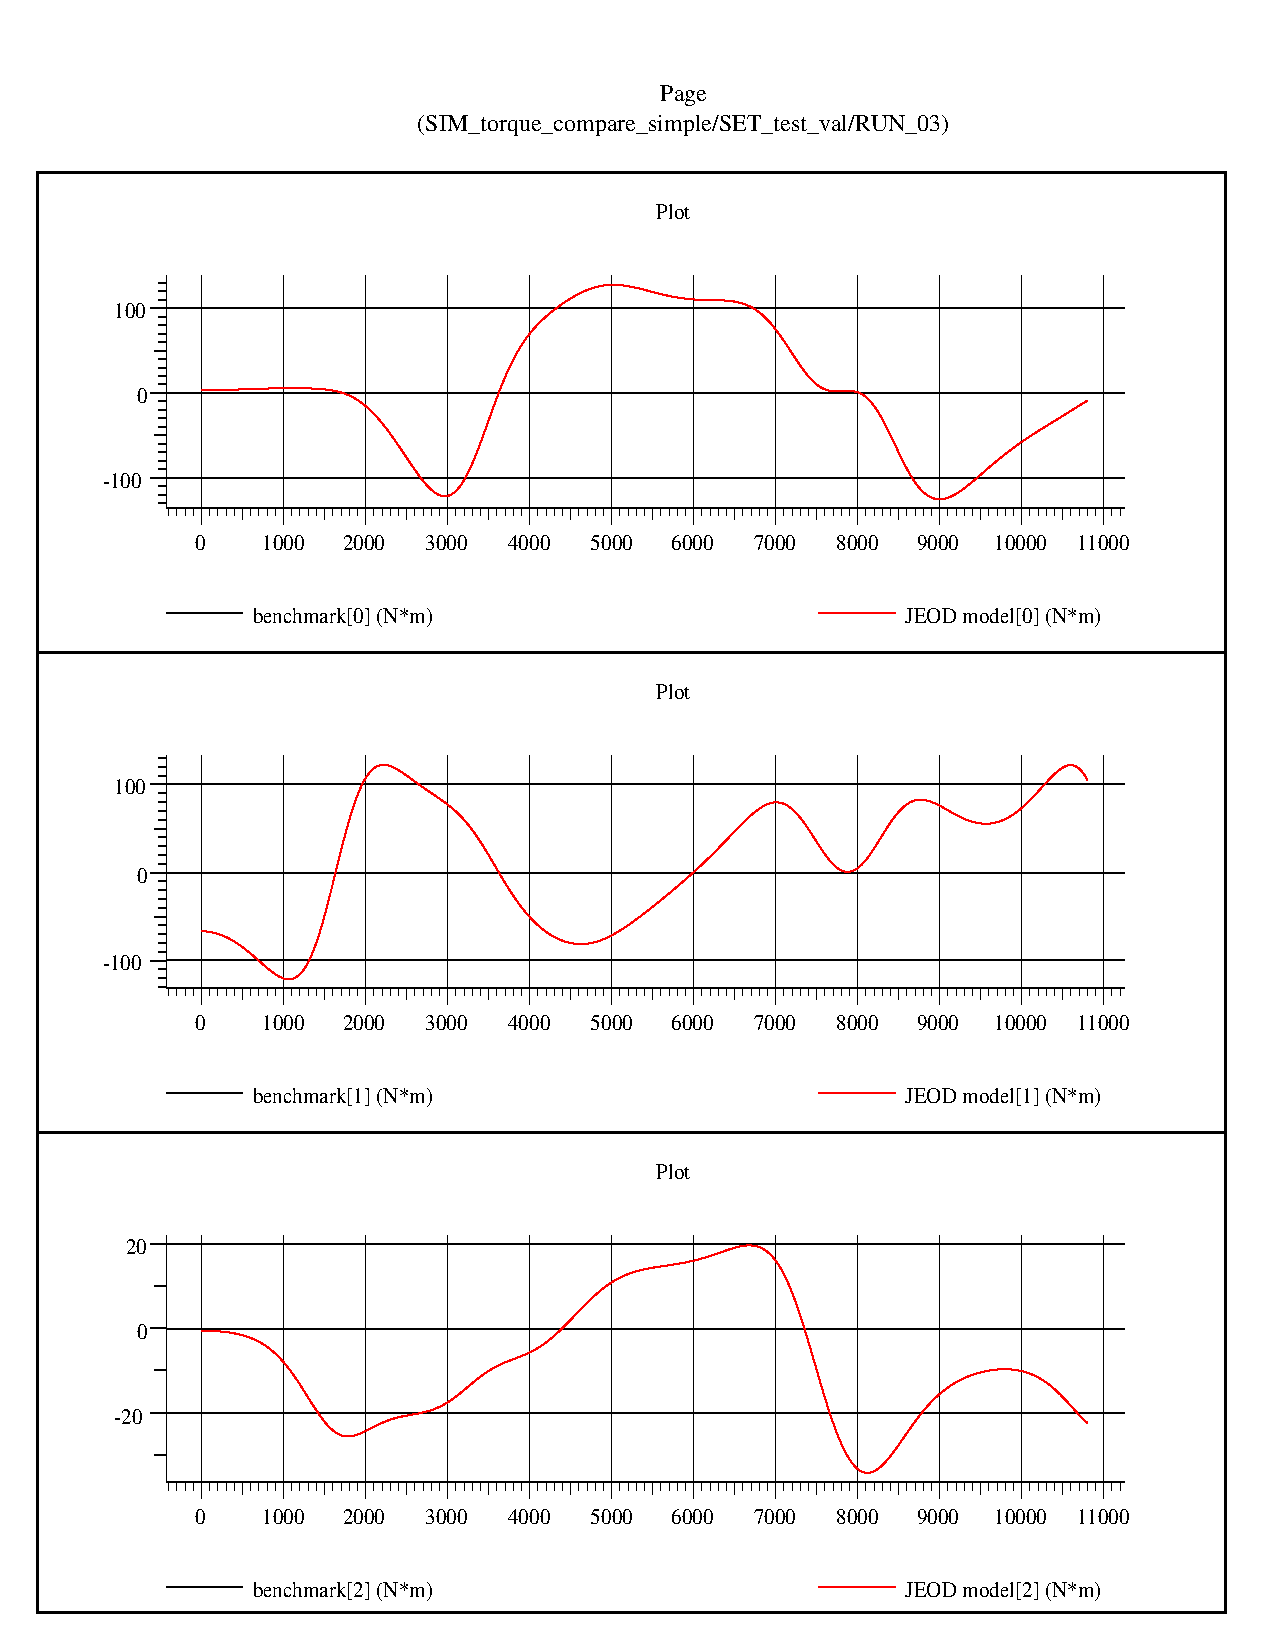
\includegraphics[width=6.1in]{figs/run_03.pdf}
\caption{RUN\_03 results.}
\label{fig:run03_results}
\end{figure}
\newpage

In the fourth sim run (RUN\_04), the Earth was  was specified to be a
non-spherical body with gravity acceleration degree and order 20.
The gravity gradient was \emph{not} activated. The input file lines
are:
\begin{verbatim}
/* Set up the gravity controls for the Earth. */
VEH_OBJ.grav_controls[0].source_name     = "Earth";
VEH_OBJ.grav_controls[0].active          = true;
VEH_OBJ.grav_controls[0].spherical       = false;
VEH_OBJ.grav_controls[0].degree          = 20;
VEH_OBJ.grav_controls[0].order           = 20;
VEH_OBJ.grav_controls[0].gradient        = false;
VEH_OBJ.grav_controls[0].gradient_degree = 0;
VEH_OBJ.grav_controls[0].gradient_order  = 0;
\end{verbatim}
The results are shown in the figure \ref{fig:run04_results}.
Because the gradient was not activated, the resulting torque
was computed to be zero in all three body frame directions 
regardless of the fact that the Earth was specified to
be non-spherical.
\begin{figure}[h!]
\centering
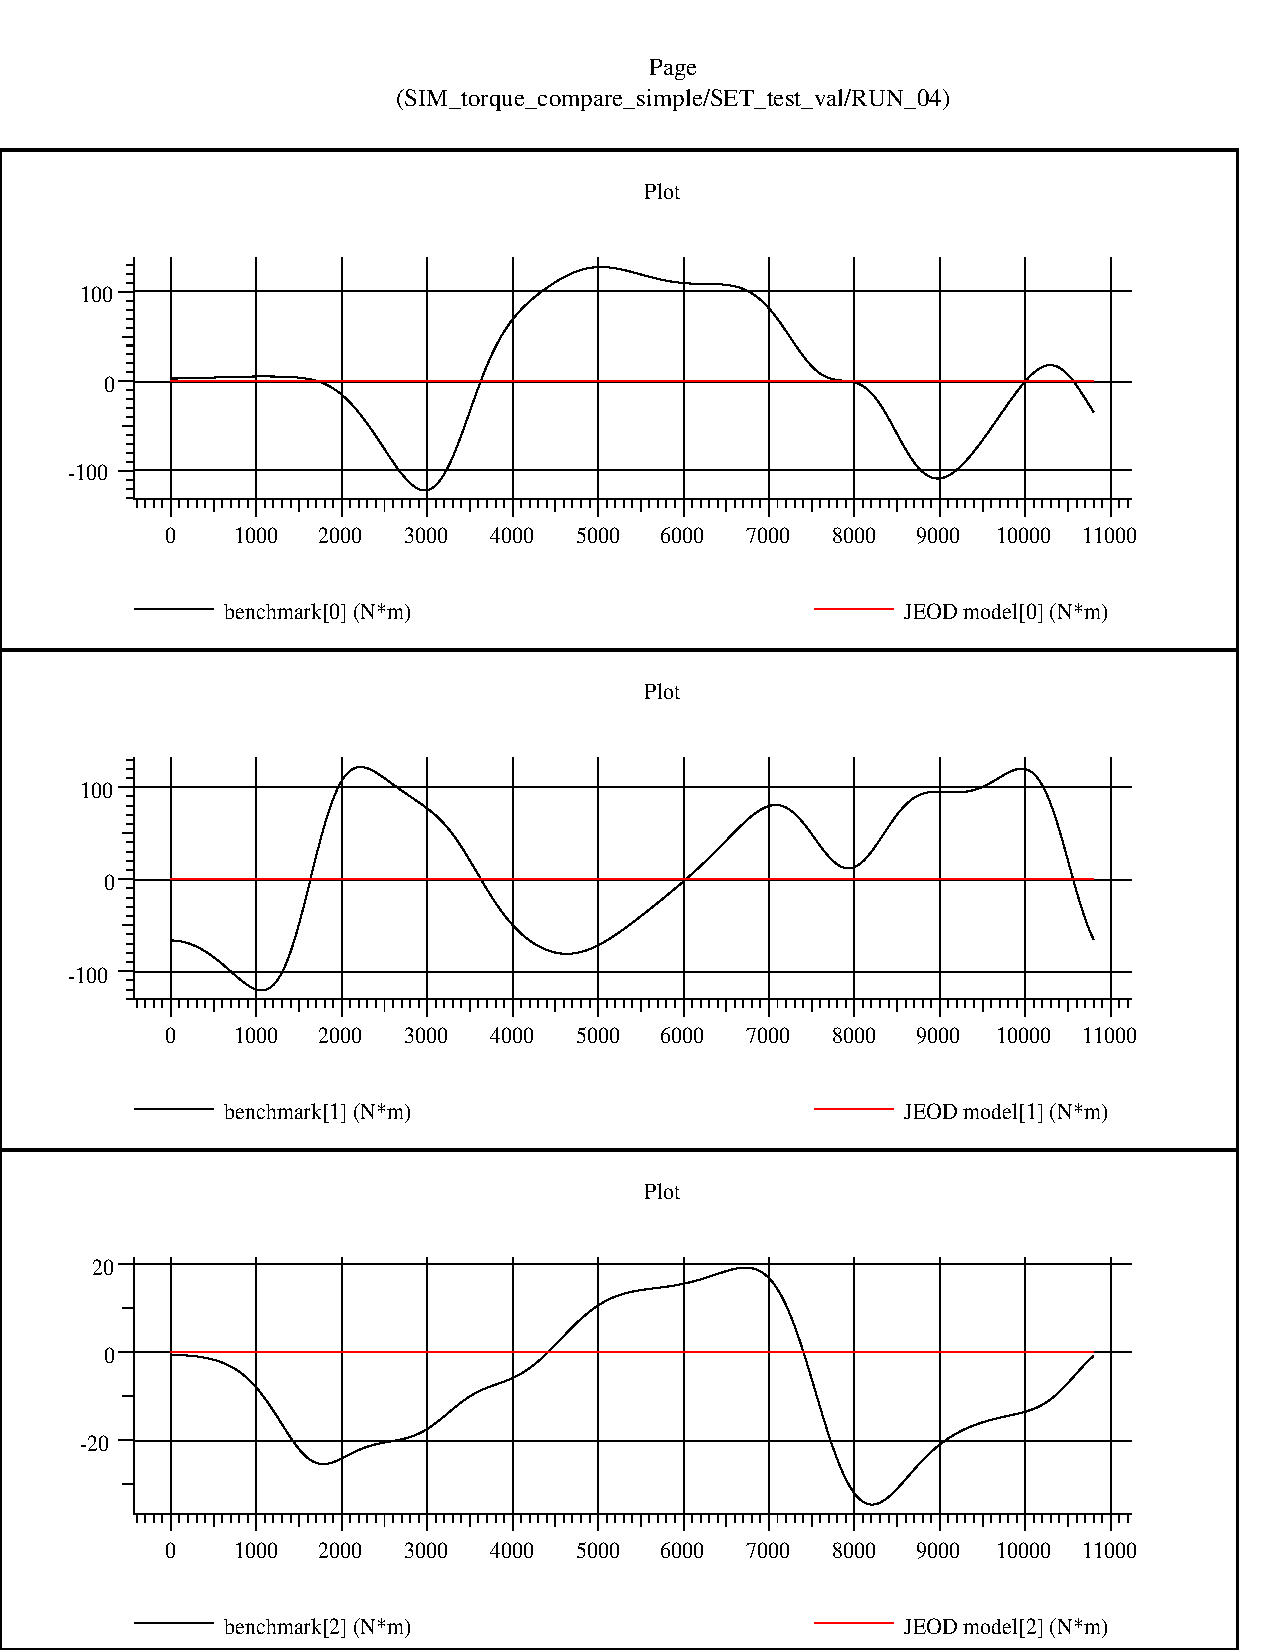
\includegraphics[width=6.1in]{figs/run_04.pdf}
\caption{RUN\_04 results.}
\label{fig:run04_results}
\end{figure}
\newpage

In the fifth sim run (RUN\_05), the Earth was specified to be a
non-spherical body with gravity acceleration degree and order 20.
The gravity gradient was activated, and the degree and order were
both specified to be 0, invoking spherical gravity gradient. 
The input file lines are:
\begin{verbatim}
/* Set up the gravity controls for the Earth. */
VEH_OBJ.grav_controls[0].source_name     = "Earth";
VEH_OBJ.grav_controls[0].active          = true;
VEH_OBJ.grav_controls[0].spherical       = false;
VEH_OBJ.grav_controls[0].degree          = 20;
VEH_OBJ.grav_controls[0].order           = 20;
VEH_OBJ.grav_controls[0].gradient        = true;
VEH_OBJ.grav_controls[0].gradient_degree = 0;
VEH_OBJ.grav_controls[0].gradient_order  = 0;
\end{verbatim}
The results are shown in the figure \ref{fig:run05_results}.
With the gradient activated and set for spherical gradient, 
the resulting torque was identical to the analytical
solution in all three body frame directions.
\begin{figure}[h!]
\centering
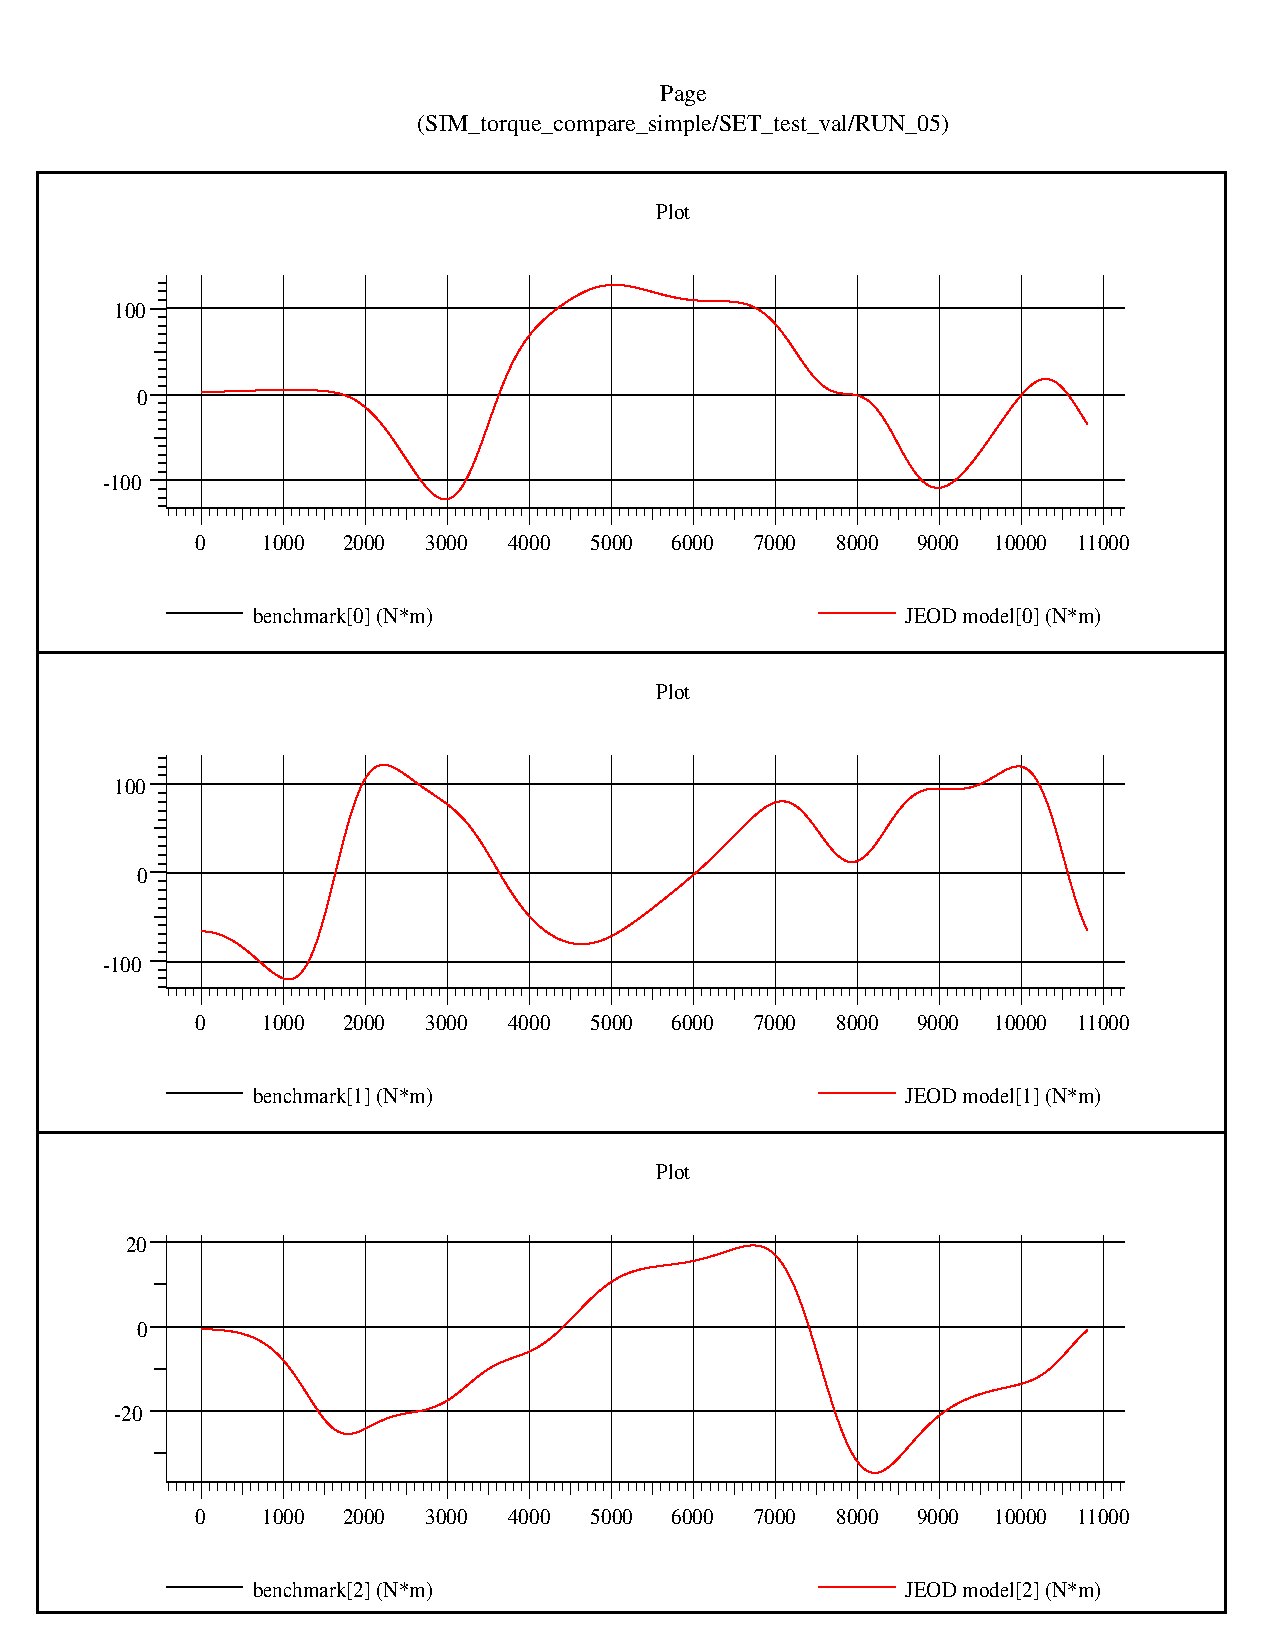
\includegraphics[width=6.1in]{figs/run_05.pdf}
\caption{RUN\_05 results.}
\label{fig:run05_results}
\end{figure}
\newpage

Finally, in the sixth sim run (RUN\_06), the Earth was specified to be a
non-spherical body with gravity acceleration degree and order 20.
The gravity gradient was activated, and the degree and order were
both specified to be 4, invoking non-spherical gravity gradient. 
The input file lines are:
\begin{verbatim}
/* Set up the gravity controls for the Earth. */
VEH_OBJ.grav_controls[0].source_name     = "Earth";
VEH_OBJ.grav_controls[0].active          = true;
VEH_OBJ.grav_controls[0].spherical       = false;
VEH_OBJ.grav_controls[0].degree          = 20;
VEH_OBJ.grav_controls[0].order           = 20;
VEH_OBJ.grav_controls[0].gradient        = true;
VEH_OBJ.grav_controls[0].gradient_degree = 4;
VEH_OBJ.grav_controls[0].gradient_order  = 4;
\end{verbatim}
A detailed sample of the results are shown in the figure \ref{fig:run06_results}.
With the gradient activated and set for non-spherical gradient, 
the resulting torque was slightly different from the analytical spherical
body torque in all three body frame directions. Whether or not the 
computed torque was the correct value was not addressed by this test.
The numerical correctness of the computations is the subject of the
next section, Validation.
\begin{figure}[h!]
\centering
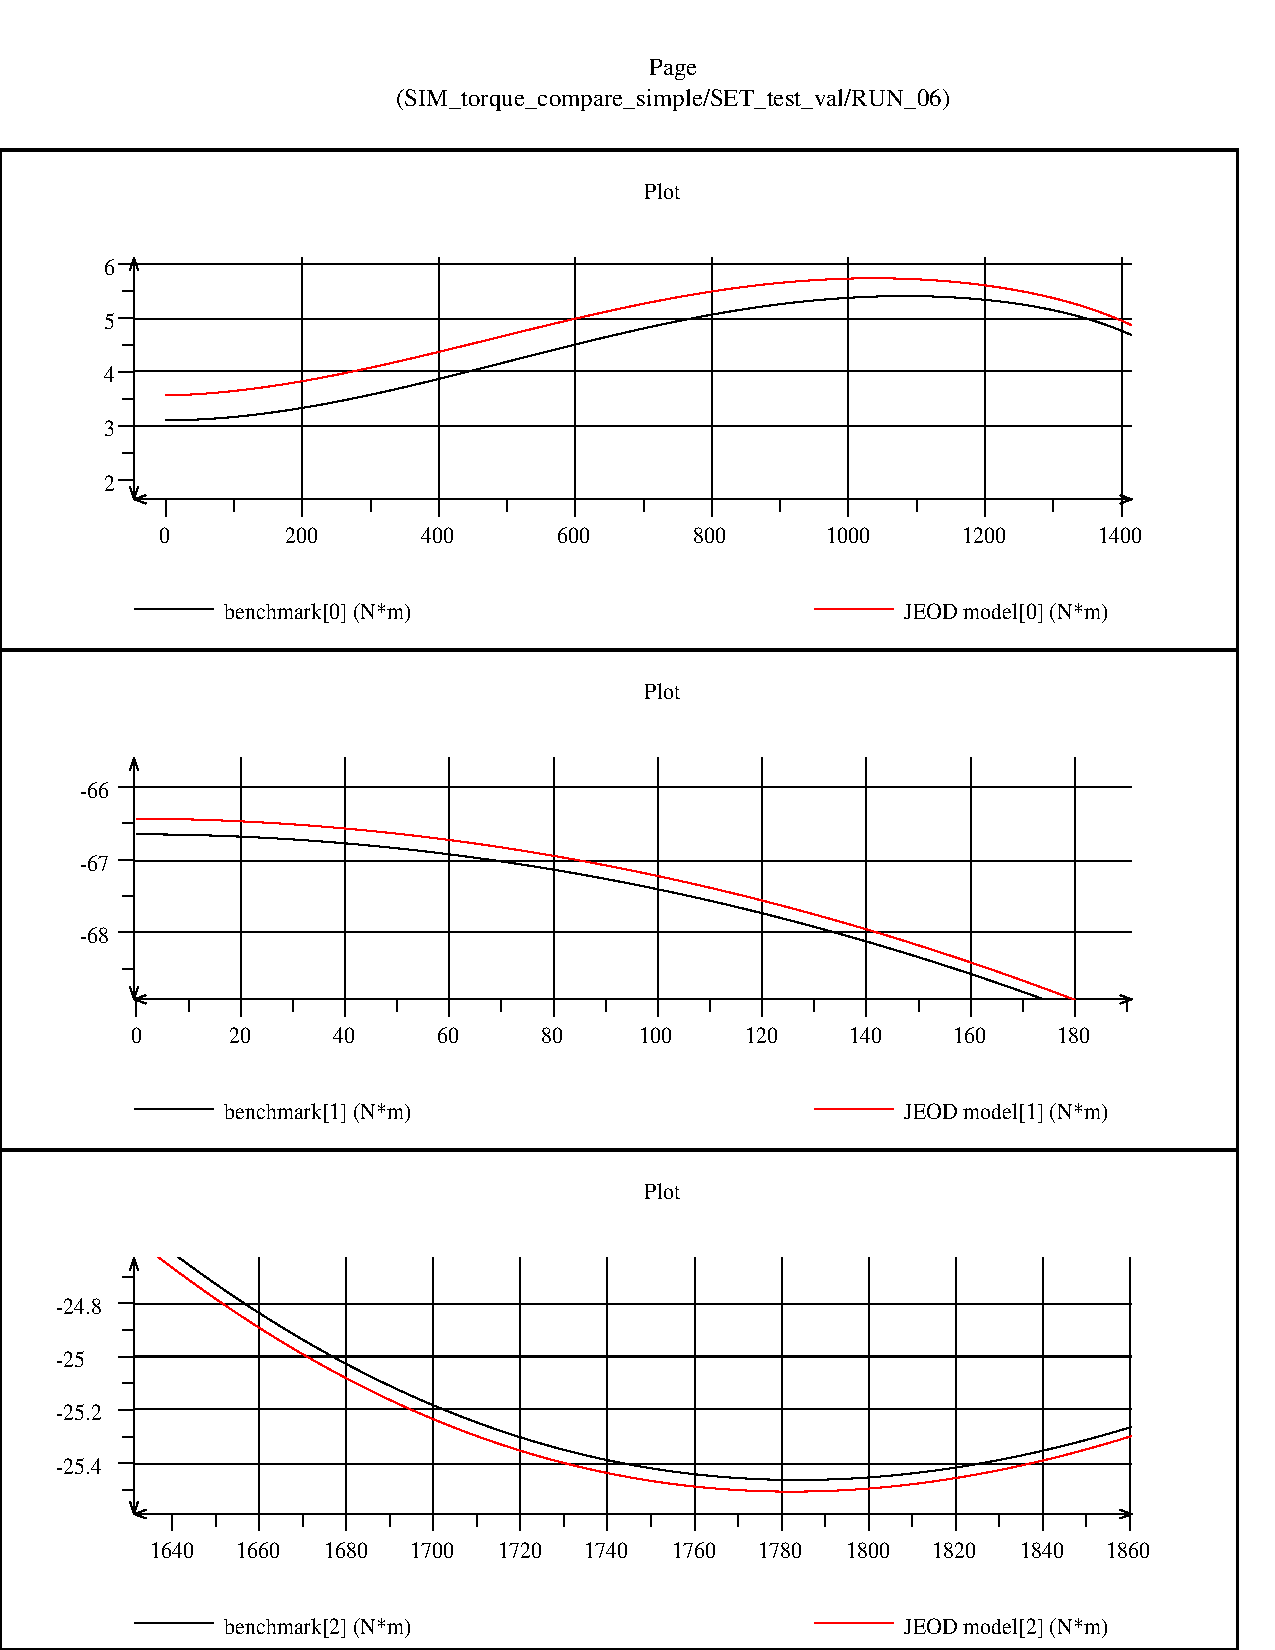
\includegraphics[width=6.1in]{figs/run_06.pdf}
\caption{RUN\_06 results (zoomed in for detail).}
\label{fig:run06_results}
\end{figure}
\newpage

%%%%%%%%%%%%%%%%%%%%%%%%%%%%%%%%%%%%%%%%%%%%%%%%%%%%%%%%%%%%%%%%%%%%%%%%%%%%%%%%
\section{Validation}\label{sec:valid}
%%% code imported from old template structure
%\test{<Title>}\label{test:<label>}
%\begin{description}
%\item[Purpose:] \ \newline
%<description>
%\item[Requirements:] \ \newline
%By passing this test, the universal time module 
%partially satisfies requirement~\ref{reqt:<label1>} and 
%completely satisfies requirement~\ref{reqt:<label2>}.
%\item[Procedure:]\ \newline
%<procedure>
%\item[Results:]\ \newline
%<results>
%\end{description}

To validate the \gravitytorqueDesc, a fictitious ``planet" was constructed
from a set of rigid point masses at known locations. The spherical harmonic
gravity coefficients representing the point mass system were 
computed and used to compute the gravity gradient by the JEOD Gravity
Model.  The gravity gradient was used as input to the 
\gravitytorqueDesc. Because the mass and location of each point of
the point mass system was known, the torque acting on the spacecraft
due to the gravity of the point masses was directly computed from 
first principles of physics. The results of this direct computation
were compared to the results of the \gravitytorqueDesc\ for validation
of the model. See Thompson {\it et al.} for details\cite{thompson2008}.

{\bf Point Mass System}

A system of 12 point masses was configured by experimentation. The 
total mass of the system was approximately equal to the mass of the 
Earth roughly divided among all of the points (see table 
\ref{pointmasses}).  The first six point masses were chosen to 
result in a center of mass at the origin and equal mass in the 
northern and southern hemispheres. The north/south symmetry of mass 
caused the odd zonal $(m=0)$ coefficients to be zero. This was 
unsuitable for evaluation of the spherical harmonic algorithms, so 
the final six point masses were included such that more mass was 
positioned in the southern hemisphere (similar to Earth). These 
points were added to the system in pairs such that the center of 
mass remained at the origin of the coordinate system in spite of the 
unequal north/south mass distribution. In terms of radial distance 
from the origin, the center of mass of two points is
\begin{equation}\label{com1}
c.o.m=\frac{r_1m_1+r_2m_2}{m_1+m_2}
\end{equation}
This assumes the masses are situated in diametrically opposing 
locations with respect to the origin. Setting equation \ref{com1} to 
zero and solving for $r_2$ yields
\begin{equation}\label{com2}
r_2=\frac{m_1}{m_2}r_1
\end{equation}
This is the radial position of the second point mass in each pair 
that kept the center of mass at the origin.

Table \ref{pointmasses} shows the 12 point masses that were 
selected.  This system resulted in degree-one gravity coefficients 
on the order of $\sim 10^{-20}$, indicating that the center of mass 
of the system was very nearly located at the origin. Therefore, the degree-one terms were 
considered negligible and forced to be exactly zero for all 
computations. This was necessary because many spherical harmonic 
algorithms make this assumption and begin computing with the 
degree-two terms.
\begin{table}\caption{Point mass model of the gravitational body.} \label{pointmasses}
\smallskip
\[ \begin{array}{| l | l | l | l | l |}\hline
\mbox{Point} & \mbox{Mass(kg)} & \mbox{Lat. (deg)} & \mbox{Lon.
(deg)} & \mbox{Radius (m)}
\\*[0.3cm]\hline \hline

\mbox{1} & \mbox{$M_\oplus/12$} & \mbox{ 45.0} & \mbox{0.0} & \mbox{4000.0} \\

\mbox{2} & \mbox{$M_\oplus/12$} & \mbox{ 45.0} & \mbox{120.0} & \mbox{4000.0} \\

\mbox{3} & \mbox{$M_\oplus/12$} & \mbox{ 45.0} & \mbox{240.0} & \mbox{4000.0} \\

\mbox{4} & \mbox{$M_\oplus/12$} & \mbox{-45.0} & \mbox{180.0} & \mbox{4000.0} \\

\mbox{5} & \mbox{$M_\oplus/12$} & \mbox{-45.0} & \mbox{300.0} & \mbox{4000.0} \\

\mbox{6} & \mbox{$M_\oplus/12$} & \mbox{-45.0} & \mbox{60.0} & \mbox{4000.0} \\

\mbox{7} & \mbox{$0.8M_\oplus/12$} & \mbox{ 23.0} & \mbox{73.0} & \mbox{4000.0} \\

\mbox{8} & \mbox{$1.2M_\oplus/12$} & \mbox{-23.0} & \mbox{253.0} & \mbox{(0.8/1.2)4000.0} \\

\mbox{9} & \mbox{$0.6M_\oplus/12$} & \mbox{ 77.0} & \mbox{303.0} & \mbox{4000.0} \\

\mbox{10} & \mbox{$1.4M_\oplus/12$} & \mbox{-77.0} & \mbox{123.0} & \mbox{(0.6/1.4)4000.0} \\

\mbox{11} & \mbox{$0.6M_\oplus/12$} & \mbox{ 51.0} & \mbox{12.0} & \mbox{4000.0} \\

\mbox{12} & \mbox{1.4$M_\oplus/12$} & \mbox{-51.0} & \mbox{192.0} & \mbox{(0.6/1.4)4000.0} \\

\hline
\end{array} \]
\end{table}

%%%%%%%%%%%%%%%%%%%%%%%%%%%%%%%%%%%%%%%%%%%%%%%%%%%%%%%%%%%%%%%%%%%%%%%%%%%%%%%%
\test{Gravity Torque Test}\label{test:gravity_torque}

To validate the \gravitytorqueDesc\, a fictitious spacecraft model 
consisting of three point masses was developed. The point masses and
locations in the body fixed frame are shown in Table \ref{table:sc_masses}.
\begin{table}\caption{Point masses and locations of the spacecraft model.} \label{table:sc_masses}
\smallskip
\[ \begin{array}{| c | c | r | r | r |}\hline
\mbox{Point} & \mbox{Mass(kg)} & \mbox{x (m)} & \mbox{y (m)} & \mbox{x (m)}
\\*[0.3cm]\hline \hline
1 & 50.0 &  1.625 &  1.250 & -1.750 \\
2 & 20.0 & -2.375 & -1.750 &  3.250 \\
3 & 10.0 & -3.375 & -2.750 &  2.250 \\
\hline
\end{array} \]
\end{table}
The equivalent
inertia tensor was
\begin{equation}
I = \left[
\begin{array}{rrr}
 630.00 & -277.50 & 372.50 \\
-277.50 &  773.75 & 285.00 \\
 372.50 &  285.00 & 573.75 \\
\end{array}
\right]
\end{equation}
For validation purposes, a pitch-yaw-roll (2-3-1) sequence was assumed.
Attitude angles of pitch = 20 deg, yaw = 30 deg, roll = 40 deg were used
for all test cases shown in table \ref{tab:testpoints}.

\begin{table}\caption{Test point locations.} \label{tab:testpoints}
\smallskip
\[ \begin{array}{| c | c | c | c |}\hline
\mbox{Test Point} & \mbox{Lat. (deg)} & \mbox{Lon. (deg)} & \mbox{Radius (m)}
\\*[0.3cm]\hline \hline
1  &  90.00 & 120.00 & 6800000.0 \\
2  &  89.99 & 353.00 & 6800000.0 \\
3  &  73.00 &   9.00 & 6800000.0 \\
4  &  13.00 & 100.00 & 6800000.0 \\
5  &   0.00 &   0.00 & 6800000.0 \\
6  &   0.00 & 180.00 & 6800000.0 \\
7  & -26.00 & 210.00 & 6800000.0 \\
8  & -52.00 & 310.00 & 6800000.0 \\
9  & -89.99 &  10.00 & 6800000.0 \\
10 & -90.00 & 160.00 & 6800000.0 \\
\hline
\end{array} \] 
\end{table}


{\bf Results}

A set of test points was selected somewhat randomly to compare the
acceleration computed by the spherical harmonic algorithms to the
point mass acceleration. All test points were selected to have a
radial distance of 6800000.0 meters, approximating the altitude of a
typical low-earth orbiting satellite.

The results in table \ref{torqueresults} show by-component differences 
typically on the order of six or more orders of magnitude smaller than
the torque magnitude. This was considered acceptable in light of the
linearity approximations used in deriving the torque model (see Gottlieb
\cite{JSC23762} p.19). 

\begin{table}\caption{Results comparing torque vectors computed by
the spherical harmonic algorithm vs. torque vectors computed 
directly from the point mass planet.} \label{torqueresults}
\smallskip
\[ \begin{array}{| c | c | c | c |}\hline
\mbox{Test Point} & \mbox{Sph. Harm. Torque} & \mbox{Pt. Mass Torque} & \mbox{Difference}
\\*[0.3cm]\hline \hline

\mbox{1} & \mbox{-6.576995906413200E-04} & \mbox{-6.576998403033940E-04} & \mbox{2.5E-10} \\
\mbox{ } & \mbox{ 1.269164209592045E-04} & \mbox{ 1.269165028503494E-04} & \mbox{8.2E-11} \\
\mbox{ } & \mbox{-4.723482089916854E-04} & \mbox{-4.723484289002045E-04} & \mbox{2.2E-10} \\
\hline

\mbox{2} & \mbox{-6.577475179730652E-04} & \mbox{-6.577477676614763E-04} & \mbox{2.5E-10} \\
\mbox{ } & \mbox{ 1.270487433086179E-04} & \mbox{ 1.270488252202995E-04} & \mbox{8.2E-11} \\
\mbox{ } & \mbox{-4.722975646974573E-04} & \mbox{-4.722977844267007E-04} & \mbox{2.2E-10} \\
\hline

\mbox{3} & \mbox{-4.667054619988188E-04} & \mbox{-4.667057505685079E-04} & \mbox{2.9E-10} \\
\mbox{ } & \mbox{ 2.230918182780193E-04} & \mbox{ 2.230919879480098E-04} & \mbox{1.7E-10} \\
\mbox{ } & \mbox{-2.308991703765578E-04} & \mbox{-2.308993437338813E-04} & \mbox{1.7E-10} \\
\hline

\mbox{4} & \mbox{ 9.643230821702463E-04} & \mbox{ 9.643234462686223E-04} & \mbox{3.6E-10} \\
\mbox{ } & \mbox{ 3.894826293977236E-04} & \mbox{ 3.894828155921459E-04} & \mbox{1.9E-10} \\
\mbox{ } & \mbox{ 1.192559213912787E-03} & \mbox{ 1.192559729815912E-03} & \mbox{5.2E-10} \\
\hline

\mbox{5} & \mbox{ 5.947635780445906E-05} & \mbox{ 5.947628430647001E-05} & \mbox{7.3E-11} \\
\mbox{ } & \mbox{-1.824208387207120E-04} & \mbox{-1.824204566105436E-04} & \mbox{3.8E-10} \\
\mbox{ } & \mbox{-1.311220703920095E-04} & \mbox{-1.311218693729188E-04} & \mbox{2.0E-10} \\
\hline

\mbox{6} & \mbox{ 5.947635779717441E-05} & \mbox{ 5.947643117565349E-05} & \mbox{7.3E-11} \\
\mbox{ } & \mbox{-1.824208387253428E-04} & \mbox{-1.824212203018760E-04} & \mbox{3.8E-10} \\
\mbox{ } & \mbox{-1.311220704109403E-04} & \mbox{-1.311222710853599E-04} & \mbox{2.0E-10} \\
\hline

\mbox{7} & \mbox{ 7.585422706336786E-04} & \mbox{ 7.585422953582111E-04} & \mbox{2.5E-11} \\
\mbox{ } & \mbox{-1.035277845536193E-03} & \mbox{-1.035277890196085E-03} & \mbox{4.5E-11} \\
\mbox{ } & \mbox{-5.060880799457042E-05} & \mbox{-5.060879752250003E-05} & \mbox{1.0E-11} \\
\hline

\mbox{8} & \mbox{ 5.494210701133441E-04} & \mbox{ 5.494212856262948E-04} & \mbox{2.2E-10} \\
\mbox{ } & \mbox{ 1.890337404179465E-04} & \mbox{ 1.890338145713599E-04} & \mbox{7.4E-11} \\
\mbox{ } & \mbox{ 6.827228269632132E-04} & \mbox{ 6.827230673707163E-04} & \mbox{2.4E-10} \\
\hline

\mbox{9} & \mbox{-6.577823003575999E-04} & \mbox{-6.577820505526688E-04} & \mbox{2.5E-10} \\
\mbox{ } & \mbox{ 1.268171069274990E-04} & \mbox{ 1.268170250483536E-04} & \mbox{8.2E-11} \\
\mbox{ } & \mbox{-4.724987427239774E-04} & \mbox{-4.724985225834644E-04} & \mbox{2.2E-10} \\
\hline

\mbox{10}& \mbox{-6.576995906610781E-04} & \mbox{-6.576993405928988E-04} & \mbox{2.5E-10} \\
\mbox{ } & \mbox{ 1.269164210444634E-04} & \mbox{ 1.269163389849837E-04} & \mbox{8.2E-11} \\
\mbox{ } & \mbox{-4.723482089531574E-04} & \mbox{-4.723479888752991E-04} & \mbox{2.2E-10} \\
\hline

\end{array} \] 
\end{table}

\newpage


\section{Requirements Traceability}\label{sec:traceability}
The table below cross-references each requirement of the 
\gravitytorqueDesc\ 
%(as defined in \href{file:GRAVITYReqt.pdf}
%{\em \GRAVITY\ Product Requirements}\cite{dynenv:GRAVITYReqt})
to a corresponding verification and/or validation test
described in sections \ref{sec:verif} and \ref{sec:valid} of this document. 

\label{tab:reqt_ivv_xref}
\begin{longtable}[c]{||p{3.5in}|p{3.5in}|}
\caption{Requirements Traceability} \\[6pt]
\hline
{\bf Requirement} & {\bf Inspection or Test} \\ \hline \hline
\endfirsthead
\hline
\endfoot
\caption[]{Requirements Traceability (continued)} \\[6pt]
\hline
{\bf Requirement} & {\bf Test} \\ \hline \hline
\endhead

\ref{reqt:gradient_matrix} - Gravity Gradient Matrix &
  Test \ref{test:gravity_torque} - Gravity Torque Test \\ \hline

\ref{reqt:mass_properties} - Spacecraft Mass Properties &
  Test \ref{test:gravity_torque} - Gravity Torque Test \\ \hline

\ref{reqt:spacecraft_attitude} - Spacecraft Attitude &
  Test \ref{test:gravity_torque} - Gravity Torque Test \\ \hline

\ref{reqt:gravity_torque} - Gravity Torque &
  Test \ref{test:gravity_torque} - Gravity Torque Test \\ \hline

\end{longtable}










%%% or for a document with multiple parts make as many copies of Chapters.tex
%%% as you have parts and use this format
%\hyperdef{part}{part1}{\part{Part 1 Title}}\label{pt1:title}
%\include{gravitytorqueChapters1}
%\hyperdef{part}{part2}{\part{Part 2 Title}}\label{pt2:title}
%\include{gravitytorqueChapters2}
%%% etc.

%%%%%%%%%%%%%%%%%%%%%%%%%%%%%%%%%%%%%%%%%%%%%%%%%%%%%%%%%%%%%%%%%%%%%%%%%
% Bibliography
%%%%%%%%%%%%%%%%%%%%%%%%%%%%%%%%%%%%%%%%%%%%%%%%%%%%%%%%%%%%%%%%%%%%%%%%%
\newpage
\pdfbookmark{Bibliography}{bibliography}
\bibliography{dynenv,gravity_torque}
\bibliographystyle{plain}

%\pagebreak
%\appendix

\end{document}
